The analog output of the AD5678-2, when using the internal $2.5\unit{V}$ voltage reference, can vary over the range of $0\unit{V}$ to $5\unit{V}$.  The output voltage is given by the equation
\begin{equation}
\label{equ:DACout}
\mathrm{Vout} = 2 \times \mathrm{VrefOut}  \times \frac{D}{2^N},
\end{equation}
where $D$ is the decimal equivalent of the binary value loaded into the DAC output register and $N$ is the resolution of the DAC (16 for the DAC outputs used on the Electrophysiology Interface board)~\cite{AD5678ds}.  It is desirable to have pulses as high as $10\unit{V}$ and with biphasic shapes to perform some electrophysiology experiments~\cite{Olivo,Kladt2010}.  Thus, some form of signal gain and offset is needed to extend the range of the output signal.  It is also desirable to be able to perform experiments with differential outputs, so the single-ended output of the DAC is converted to a differential output.

The design of Differential Output Amplifier circuit as shown in Figure~\ref{fig:DiffAmp} consists of a difference amplifier circuit, implemented with operational amplifier (op-amp) OA1, to perform the gain and offset operations on the DAC output and an inverting amplifier, implemented with op-amp OA2, to create a differential output.  The Differential Output Amplifier design is replicated for each of the DAC outputs to create four unique outputs that can be connected to stimulation electrodes single-endedly (between Vout+ and AGND or $\mathrm{Vout-}$ and AGND) or differentially (between Vout+ and $\mathrm{Vout-}$).

\begin{figure}[H]
	\centering 
		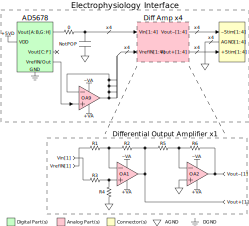
\includegraphics{./figures/DiffAmp} 
	\caption{Differential Output Amplifier\label{fig:DiffAmp}}
\end{figure}

The difference amplifier op-amp configuration is well known, with its operation described by equation
\begin{equation}
\label{equ:DifferenceAmp1}
\mathrm{Vout+} = \frac{R_2}{R_1} \frac{1 + R_1/R_2}{1 + R_3/R_4} \mathrm{Vin} - \frac{R_2}{R_1} \mathrm{VrefIN};
\end{equation}
choosing resistor values with the constraint
\begin{equation}
\label{equ:DifferenceAmp2}
\frac{R_1}{R_2}  = \frac{R_3}{R_4} 
\end{equation}
yields the simpler form
\begin{equation}
\label{equ:DifferenceAmp3}
\mathrm{Vout+} = \frac{R_2}{R_1} (\mathrm{Vin} - \mathrm{VrefIN}),
\end{equation}
which has the gain and offset elements needed to fulfill the design requirements~\cite{AlexanderSadiku2004}.

The $0\unit{V}$ to $5\unit{V}$ range of the DAC outputs can be made symmetrical around $0\unit{V}$ by subtracting $2.5\unit{V}$, yielding a range of $-2.5\unit{V}$ to $2.5\unit{V}$.  Thus, the range of Vout+ is $-2.5\unit{V}  \times R_2/R_1$ to $2.5\unit{V} \times R_2/R_1$, allowing the output range to be easily calculated and changed if needed.  Since the AD5678 makes its internal $2.5\unit{V}$ voltage reference accessible on an external pin, using that voltage as an input to the difference amplifier eliminates the need for an external voltage reference circuit that would involve a resistor network susceptible to inaccuracies in the power supply voltage or a specialized voltage reference IC.  Substituting the midscale DAC code 0x7FFF into equation~\eqref{equ:DACout} and~\eqref{equ:DifferenceAmp3} yields $\mathrm{Vout+}=76 \unit{\mu V} \times R_2/R_1$ which is very close to $0\unit{V}$.  Programming the AD5678 to output midscale codes on the DAC outputs after power-on reset will ensure than stimulation electrodes have a low DC voltage without having to write the DAC code at every power cycle.

An inverted output is needed to implement a differential output amplifier.  This can be accomplished with an op-amp in an inverting configuration.  The equation for the inverting amplifier is \begin{equation}
\label{equ:InvertingAmp1}
\mathrm{Vout-} = -\frac{R_6}{R_5} \mathrm{Vout+} ;
\end{equation}
choosing $R_5 = R_6$ will make $\mathrm{Vout-}$ the inverse of Vout+~\cite{AlexanderSadiku2004}.  The ratio $R_2/R_1$ is set to $3$ to produce single-ended output range of $-2.5\unit{V}  \times R_2/R_1$ to $2.5\unit{V} \times R_2/R_1  \Rightarrow -7.5\unit{V}$ to $7.5\unit{V}$, which will be close to the saturation voltages of an op-amp powered from $\pm 9\unit{V}$ supplies.  Table~\ref{tab:DiffOutAmpRes} shows resistor values chosen and calculated for the design.

\renewcommand{\arraystretch}{1.3}
\begin{table}[h]
\centering 
\begin{tabular}{l l l l}
\hline
Choose	& $R_1$	& $R_3$ & $R_2/R_1$	\\
	&	$1\unit{k\Omega}$	&  $1\unit{k\Omega}$ &	$3$	\\
Yields	& $R_2$ &  $R_4$ &	\\
	&	$3\unit{k\Omega}$	& $3\unit{k\Omega}$ &	\\
\hline
Choose	& $R_5$ &	&	\\
	&	$1\unit{k\Omega}$	& 	&	\\
Yields	& $R_6$ &  & 	\\
	&	$1\unit{k\Omega}$	&	&	\\
\hline
\end{tabular}
\caption{Resistor values for the Differential Output Amplifier\label{tab:DiffOutAmpRes} }

\end{table}
\renewcommand{\arraystretch}{1.0}

The dual packaged LT1124-1 precision op-amp from Linear Technology\textsuperscript{\textregistered} was chosen because the LT1124/LT1125 part family was used in~\cite{StahlMSEE,BatzerCorsiCrampton}, SPICE amplifier models are available for LTspice\textsuperscript{\textregistered} circuit simulation software, the dual package allows the Differential Output Amplifier block with two op-amps to be implemented with only one IC, and the -1 option specifies a standard pinout 8-SO surface mount part so other op-amp models may be tested with the design~\cite{LT11245ds}.

According to~\cite{AD5678ds}, the voltage reference output should be buffered if used to drive a load, so a single op-amp in a voltage follower configuration is used to buffer the reference voltage to the Differential Output Amplifier blocks.  One half of an LT1124-1 is used to be consistent with the other op-amps on the Electrophysiology Interface board.  The buffer op-amp, OA9, drives current through $R_1$ of the Differential Output Amplifier block; thus, the op-amp will need to be capable of driving current to four amplifier blocks.  The maximum current the OA9 will need to provide will be determined by the maximum voltage across $R_1$ multiplied by four.  The maximum voltage across $R_1$ will be when Vin equals $0\unit{V}$, which would yield a maximum current of $(\mathrm{Vref}-0\unit{V})/R_1\times4=2.5\unit{V}/1\unit{k\Omega} \times4=10\unit{mA}$.  It may be necessary to choose higher value resistors if the buffer is needed to drive more amplifier blocks or it is seen that the output voltage of OA9 changes during use.

The design of the Differential Output Amplifier was entered into the circuit simulation program LTspice\textsuperscript{\textregistered}, as shown in Figure~\ref{fig:DiffAmp}, to test the design of the circuit.  The first test performed was a DC sweep of Vin to display the transfer function from the outputs Vout+ and $\mathrm{Vout-}$.  The transfer function is shown in Figure~\ref{fig:DCSweep}.  Saturation occurs at $40\unit{mV}$ and $4.95\unit{V}$ yielding saturation voltages of approximately $\pm7.4\unit{V}$, allowing for almost the entire range of DAC output to be in the linear region and yielding a maximum possible output voltage, if taken differentially, of $14.8\unit{V}$.

\begin{figure}[H]
	\centering 
		\includegraphics{./figures/LTSchem} 
	\caption{LTspice\textsuperscript{\textregistered} schematic of the Differential Output Amplifier circuit\label{fig:DiffAmp}}
\end{figure}

\begin{figure}[H]
	\centering 
		\resizebox{\textwidth-0.5in}{!}{% GNUPLOT: LaTeX picture with Postscript
\begingroup
  \makeatletter
  \providecommand\color[2][]{%
    \GenericError{(gnuplot) \space\space\space\@spaces}{%
      Package color not loaded in conjunction with
      terminal option `colourtext'%
    }{See the gnuplot documentation for explanation.%
    }{Either use 'blacktext' in gnuplot or load the package
      color.sty in LaTeX.}%
    \renewcommand\color[2][]{}%
  }%
  \providecommand\includegraphics[2][]{%
    \GenericError{(gnuplot) \space\space\space\@spaces}{%
      Package graphicx or graphics not loaded%
    }{See the gnuplot documentation for explanation.%
    }{The gnuplot epslatex terminal needs graphicx.sty or graphics.sty.}%
    \renewcommand\includegraphics[2][]{}%
  }%
  \providecommand\rotatebox[2]{#2}%
  \@ifundefined{ifGPcolor}{%
    \newif\ifGPcolor
    \GPcolorfalse
  }{}%
  \@ifundefined{ifGPblacktext}{%
    \newif\ifGPblacktext
    \GPblacktexttrue
  }{}%
  % define a \g@addto@macro without @ in the name:
  \let\gplgaddtomacro\g@addto@macro
  % define empty templates for all commands taking text:
  \gdef\gplbacktext{}%
  \gdef\gplfronttext{}%
  \makeatother
  \ifGPblacktext
    % no textcolor at all
    \def\colorrgb#1{}%
    \def\colorgray#1{}%
  \else
    % gray or color?
    \ifGPcolor
      \def\colorrgb#1{\color[rgb]{#1}}%
      \def\colorgray#1{\color[gray]{#1}}%
      \expandafter\def\csname LTw\endcsname{\color{white}}%
      \expandafter\def\csname LTb\endcsname{\color{black}}%
      \expandafter\def\csname LTa\endcsname{\color{black}}%
      \expandafter\def\csname LT0\endcsname{\color[rgb]{1,0,0}}%
      \expandafter\def\csname LT1\endcsname{\color[rgb]{0,1,0}}%
      \expandafter\def\csname LT2\endcsname{\color[rgb]{0,0,1}}%
      \expandafter\def\csname LT3\endcsname{\color[rgb]{1,0,1}}%
      \expandafter\def\csname LT4\endcsname{\color[rgb]{0,1,1}}%
      \expandafter\def\csname LT5\endcsname{\color[rgb]{1,1,0}}%
      \expandafter\def\csname LT6\endcsname{\color[rgb]{0,0,0}}%
      \expandafter\def\csname LT7\endcsname{\color[rgb]{1,0.3,0}}%
      \expandafter\def\csname LT8\endcsname{\color[rgb]{0.5,0.5,0.5}}%
    \else
      % gray
      \def\colorrgb#1{\color{black}}%
      \def\colorgray#1{\color[gray]{#1}}%
      \expandafter\def\csname LTw\endcsname{\color{white}}%
      \expandafter\def\csname LTb\endcsname{\color{black}}%
      \expandafter\def\csname LTa\endcsname{\color{black}}%
      \expandafter\def\csname LT0\endcsname{\color{black}}%
      \expandafter\def\csname LT1\endcsname{\color{black}}%
      \expandafter\def\csname LT2\endcsname{\color{black}}%
      \expandafter\def\csname LT3\endcsname{\color{black}}%
      \expandafter\def\csname LT4\endcsname{\color{black}}%
      \expandafter\def\csname LT5\endcsname{\color{black}}%
      \expandafter\def\csname LT6\endcsname{\color{black}}%
      \expandafter\def\csname LT7\endcsname{\color{black}}%
      \expandafter\def\csname LT8\endcsname{\color{black}}%
    \fi
  \fi
  \setlength{\unitlength}{0.0500bp}%
  \begin{picture}(11520.00,8640.00)%
    \gplgaddtomacro\gplbacktext{%
      \csname LTb\endcsname%
      \put(620,640){\makebox(0,0)[r]{\strut{}-8}}%
      \csname LTb\endcsname%
      \put(620,1102){\makebox(0,0)[r]{\strut{}-7}}%
      \csname LTb\endcsname%
      \put(620,1565){\makebox(0,0)[r]{\strut{}-6}}%
      \csname LTb\endcsname%
      \put(620,2027){\makebox(0,0)[r]{\strut{}-5}}%
      \csname LTb\endcsname%
      \put(620,2490){\makebox(0,0)[r]{\strut{}-4}}%
      \csname LTb\endcsname%
      \put(620,2952){\makebox(0,0)[r]{\strut{}-3}}%
      \csname LTb\endcsname%
      \put(620,3415){\makebox(0,0)[r]{\strut{}-2}}%
      \csname LTb\endcsname%
      \put(620,3877){\makebox(0,0)[r]{\strut{}-1}}%
      \csname LTb\endcsname%
      \put(620,4340){\makebox(0,0)[r]{\strut{}0}}%
      \csname LTb\endcsname%
      \put(620,4802){\makebox(0,0)[r]{\strut{}1}}%
      \csname LTb\endcsname%
      \put(620,5264){\makebox(0,0)[r]{\strut{}2}}%
      \csname LTb\endcsname%
      \put(620,5727){\makebox(0,0)[r]{\strut{}3}}%
      \csname LTb\endcsname%
      \put(620,6189){\makebox(0,0)[r]{\strut{}4}}%
      \csname LTb\endcsname%
      \put(620,6652){\makebox(0,0)[r]{\strut{}5}}%
      \csname LTb\endcsname%
      \put(620,7114){\makebox(0,0)[r]{\strut{}6}}%
      \csname LTb\endcsname%
      \put(620,7577){\makebox(0,0)[r]{\strut{}7}}%
      \csname LTb\endcsname%
      \put(620,8039){\makebox(0,0)[r]{\strut{}8}}%
      \csname LTb\endcsname%
      \put(740,440){\makebox(0,0){\strut{}-0.5}}%
      \csname LTb\endcsname%
      \put(1608,440){\makebox(0,0){\strut{}0}}%
      \csname LTb\endcsname%
      \put(2477,440){\makebox(0,0){\strut{}0.5}}%
      \csname LTb\endcsname%
      \put(3345,440){\makebox(0,0){\strut{}1}}%
      \csname LTb\endcsname%
      \put(4213,440){\makebox(0,0){\strut{}1.5}}%
      \csname LTb\endcsname%
      \put(5081,440){\makebox(0,0){\strut{}2}}%
      \csname LTb\endcsname%
      \put(5950,440){\makebox(0,0){\strut{}2.5}}%
      \csname LTb\endcsname%
      \put(6818,440){\makebox(0,0){\strut{}3}}%
      \csname LTb\endcsname%
      \put(7686,440){\makebox(0,0){\strut{}3.5}}%
      \csname LTb\endcsname%
      \put(8554,440){\makebox(0,0){\strut{}4}}%
      \csname LTb\endcsname%
      \put(9423,440){\makebox(0,0){\strut{}4.5}}%
      \csname LTb\endcsname%
      \put(10291,440){\makebox(0,0){\strut{}5}}%
      \csname LTb\endcsname%
      \put(11159,440){\makebox(0,0){\strut{}5.5}}%
      \colorrgb{0.00,0.00,0.00}%
      \put(160,4339){\rotatebox{90}{\makebox(0,0){\strut{}Voltage ($V$)}}}%
      \colorrgb{0.00,0.00,0.00}%
      \put(5949,140){\makebox(0,0){\strut{}Voltage ($V$)}}%
      \csname LTb\endcsname%
      \put(5949,8339){\makebox(0,0){\strut{}DC Sweep of Differential Output Amplifier Input $Vin$}}%
    }%
    \gplgaddtomacro\gplfronttext{%
      \csname LTb\endcsname%
      \put(10256,4439){\makebox(0,0)[r]{\strut{}$Vout+$}}%
      \csname LTb\endcsname%
      \put(10256,4239){\makebox(0,0)[r]{\strut{}$Vout-$}}%
    }%
    \gplbacktext
    \put(0,0){\includegraphics{DCSweep}}%
    \gplfronttext
  \end{picture}%
\endgroup
}
	\caption{DC Transfer Function of the Differential Output Amplifier obtained using LTspice\textsuperscript{\textregistered}\label{fig:DCSweep}}
\end{figure}

A transient simulation of a waveform used in~\cite{Olivo} was also performed.  Figure~\ref{fig:DiffAmpTransSchem} shows the output connected to single-ended loads $Rse1$ and $Rse2$ and differential load $Rd$.  A $0.2\unit{ms}$ wide pulse from midscale DAC output to an amplitude of $1.5\unit{V}$ with a slew rate of $1.5\unit{V}/ \unit{\mu s}$~\cite{AD5678ds} was simulated as a DAC output.  The input waveform and differential and single ended outputs are shown in Figure~\ref{fig:DiffAmpTransSim}.

\begin{figure}[H]
	\begin{singlespace}
	\centering 
		\includegraphics{./figures/LTSchemTrans} 
	\caption{LTspice\textsuperscript{\textregistered} schematic of the Differential Output Amplifier for transient response simulation with single-ended load resistors $Rse1$ and $Rse2$ and differential load resistor $Rd$\label{fig:DiffAmpTransSchem}}
	\end{singlespace}
\end{figure}

\begin{figure}[H]
	\begin{singlespace}
	\centering 
		\resizebox{\textwidth-0.5in}{!}{% GNUPLOT: LaTeX picture with Postscript
\begingroup
  \makeatletter
  \providecommand\color[2][]{%
    \GenericError{(gnuplot) \space\space\space\@spaces}{%
      Package color not loaded in conjunction with
      terminal option `colourtext'%
    }{See the gnuplot documentation for explanation.%
    }{Either use 'blacktext' in gnuplot or load the package
      color.sty in LaTeX.}%
    \renewcommand\color[2][]{}%
  }%
  \providecommand\includegraphics[2][]{%
    \GenericError{(gnuplot) \space\space\space\@spaces}{%
      Package graphicx or graphics not loaded%
    }{See the gnuplot documentation for explanation.%
    }{The gnuplot epslatex terminal needs graphicx.sty or graphics.sty.}%
    \renewcommand\includegraphics[2][]{}%
  }%
  \providecommand\rotatebox[2]{#2}%
  \@ifundefined{ifGPcolor}{%
    \newif\ifGPcolor
    \GPcolorfalse
  }{}%
  \@ifundefined{ifGPblacktext}{%
    \newif\ifGPblacktext
    \GPblacktexttrue
  }{}%
  % define a \g@addto@macro without @ in the name:
  \let\gplgaddtomacro\g@addto@macro
  % define empty templates for all commands taking text:
  \gdef\gplbacktext{}%
  \gdef\gplfronttext{}%
  \makeatother
  \ifGPblacktext
    % no textcolor at all
    \def\colorrgb#1{}%
    \def\colorgray#1{}%
  \else
    % gray or color?
    \ifGPcolor
      \def\colorrgb#1{\color[rgb]{#1}}%
      \def\colorgray#1{\color[gray]{#1}}%
      \expandafter\def\csname LTw\endcsname{\color{white}}%
      \expandafter\def\csname LTb\endcsname{\color{black}}%
      \expandafter\def\csname LTa\endcsname{\color{black}}%
      \expandafter\def\csname LT0\endcsname{\color[rgb]{1,0,0}}%
      \expandafter\def\csname LT1\endcsname{\color[rgb]{0,1,0}}%
      \expandafter\def\csname LT2\endcsname{\color[rgb]{0,0,1}}%
      \expandafter\def\csname LT3\endcsname{\color[rgb]{1,0,1}}%
      \expandafter\def\csname LT4\endcsname{\color[rgb]{0,1,1}}%
      \expandafter\def\csname LT5\endcsname{\color[rgb]{1,1,0}}%
      \expandafter\def\csname LT6\endcsname{\color[rgb]{0,0,0}}%
      \expandafter\def\csname LT7\endcsname{\color[rgb]{1,0.3,0}}%
      \expandafter\def\csname LT8\endcsname{\color[rgb]{0.5,0.5,0.5}}%
    \else
      % gray
      \def\colorrgb#1{\color{black}}%
      \def\colorgray#1{\color[gray]{#1}}%
      \expandafter\def\csname LTw\endcsname{\color{white}}%
      \expandafter\def\csname LTb\endcsname{\color{black}}%
      \expandafter\def\csname LTa\endcsname{\color{black}}%
      \expandafter\def\csname LT0\endcsname{\color{black}}%
      \expandafter\def\csname LT1\endcsname{\color{black}}%
      \expandafter\def\csname LT2\endcsname{\color{black}}%
      \expandafter\def\csname LT3\endcsname{\color{black}}%
      \expandafter\def\csname LT4\endcsname{\color{black}}%
      \expandafter\def\csname LT5\endcsname{\color{black}}%
      \expandafter\def\csname LT6\endcsname{\color{black}}%
      \expandafter\def\csname LT7\endcsname{\color{black}}%
      \expandafter\def\csname LT8\endcsname{\color{black}}%
    \fi
  \fi
  \setlength{\unitlength}{0.0500bp}%
  \begin{picture}(11520.00,8640.00)%
    \gplgaddtomacro\gplbacktext{%
      \colorrgb{0.00,0.00,0.00}%
      \put(1377,5312){\makebox(0,0)[r]{\strut{}0}}%
      \colorrgb{0.00,0.00,0.00}%
      \put(1377,5848){\makebox(0,0)[r]{\strut{}1}}%
      \colorrgb{0.00,0.00,0.00}%
      \put(1377,6384){\makebox(0,0)[r]{\strut{}2}}%
      \colorrgb{0.00,0.00,0.00}%
      \put(1377,6919){\makebox(0,0)[r]{\strut{}3}}%
      \colorrgb{0.00,0.00,0.00}%
      \put(1377,7455){\makebox(0,0)[r]{\strut{}4}}%
      \colorrgb{0.00,0.00,0.00}%
      \put(1377,7991){\makebox(0,0)[r]{\strut{}5}}%
      \colorrgb{0.00,0.00,0.00}%
      \put(1497,4844){\makebox(0,0){\strut{}0}}%
      \colorrgb{0.00,0.00,0.00}%
      \put(2140,4844){\makebox(0,0){\strut{}0.1}}%
      \colorrgb{0.00,0.00,0.00}%
      \put(2782,4844){\makebox(0,0){\strut{}0.2}}%
      \colorrgb{0.00,0.00,0.00}%
      \put(3425,4844){\makebox(0,0){\strut{}0.3}}%
      \colorrgb{0.00,0.00,0.00}%
      \put(4067,4844){\makebox(0,0){\strut{}0.4}}%
      \colorrgb{0.00,0.00,0.00}%
      \put(4710,4844){\makebox(0,0){\strut{}0.5}}%
      \colorrgb{0.00,0.00,0.00}%
      \put(5352,4844){\makebox(0,0){\strut{}0.6}}%
      \colorrgb{0.00,0.00,0.00}%
      \put(1037,6517){\rotatebox{90}{\makebox(0,0){\strut{}Voltage ($V$)}}}%
      \colorrgb{0.00,0.00,0.00}%
      \put(3424,4544){\makebox(0,0){\strut{}Time ($ms$)}}%
      \csname LTb\endcsname%
      \put(3424,8291){\makebox(0,0){\strut{}Input Voltage $Vin$}}%
    }%
    \gplgaddtomacro\gplfronttext{%
    }%
    \gplgaddtomacro\gplbacktext{%
      \colorrgb{0.00,0.00,0.00}%
      \put(6450,5312){\makebox(0,0)[r]{\strut{}0}}%
      \colorrgb{0.00,0.00,0.00}%
      \put(6450,5848){\makebox(0,0)[r]{\strut{}2}}%
      \colorrgb{0.00,0.00,0.00}%
      \put(6450,6384){\makebox(0,0)[r]{\strut{}4}}%
      \colorrgb{0.00,0.00,0.00}%
      \put(6450,6919){\makebox(0,0)[r]{\strut{}6}}%
      \colorrgb{0.00,0.00,0.00}%
      \put(6450,7455){\makebox(0,0)[r]{\strut{}8}}%
      \colorrgb{0.00,0.00,0.00}%
      \put(6450,7991){\makebox(0,0)[r]{\strut{}10}}%
      \colorrgb{0.00,0.00,0.00}%
      \put(6570,4844){\makebox(0,0){\strut{}0}}%
      \colorrgb{0.00,0.00,0.00}%
      \put(7212,4844){\makebox(0,0){\strut{}0.1}}%
      \colorrgb{0.00,0.00,0.00}%
      \put(7855,4844){\makebox(0,0){\strut{}0.2}}%
      \colorrgb{0.00,0.00,0.00}%
      \put(8497,4844){\makebox(0,0){\strut{}0.3}}%
      \colorrgb{0.00,0.00,0.00}%
      \put(9139,4844){\makebox(0,0){\strut{}0.4}}%
      \colorrgb{0.00,0.00,0.00}%
      \put(9782,4844){\makebox(0,0){\strut{}0.5}}%
      \colorrgb{0.00,0.00,0.00}%
      \put(10424,4844){\makebox(0,0){\strut{}0.6}}%
      \colorrgb{0.00,0.00,0.00}%
      \put(5990,6517){\rotatebox{90}{\makebox(0,0){\strut{}Voltage ($V$)}}}%
      \colorrgb{0.00,0.00,0.00}%
      \put(8497,4544){\makebox(0,0){\strut{}Time ($ms$)}}%
      \csname LTb\endcsname%
      \put(8497,8291){\makebox(0,0){\strut{}Differential Output Voltage $Vout+$ to $Vout-$}}%
    }%
    \gplgaddtomacro\gplfronttext{%
    }%
    \gplgaddtomacro\gplbacktext{%
      \colorrgb{0.00,0.00,0.00}%
      \put(1377,1161){\makebox(0,0)[r]{\strut{}-6}}%
      \colorrgb{0.00,0.00,0.00}%
      \put(1377,1582){\makebox(0,0)[r]{\strut{}-4}}%
      \colorrgb{0.00,0.00,0.00}%
      \put(1377,2003){\makebox(0,0)[r]{\strut{}-2}}%
      \colorrgb{0.00,0.00,0.00}%
      \put(1377,2424){\makebox(0,0)[r]{\strut{}0}}%
      \colorrgb{0.00,0.00,0.00}%
      \put(1377,2845){\makebox(0,0)[r]{\strut{}2}}%
      \colorrgb{0.00,0.00,0.00}%
      \put(1377,3266){\makebox(0,0)[r]{\strut{}4}}%
      \colorrgb{0.00,0.00,0.00}%
      \put(1377,3687){\makebox(0,0)[r]{\strut{}6}}%
      \colorrgb{0.00,0.00,0.00}%
      \put(1497,750){\makebox(0,0){\strut{}0}}%
      \colorrgb{0.00,0.00,0.00}%
      \put(2140,750){\makebox(0,0){\strut{}0.1}}%
      \colorrgb{0.00,0.00,0.00}%
      \put(2782,750){\makebox(0,0){\strut{}0.2}}%
      \colorrgb{0.00,0.00,0.00}%
      \put(3425,750){\makebox(0,0){\strut{}0.3}}%
      \colorrgb{0.00,0.00,0.00}%
      \put(4067,750){\makebox(0,0){\strut{}0.4}}%
      \colorrgb{0.00,0.00,0.00}%
      \put(4710,750){\makebox(0,0){\strut{}0.5}}%
      \colorrgb{0.00,0.00,0.00}%
      \put(5352,750){\makebox(0,0){\strut{}0.6}}%
      \colorrgb{0.00,0.00,0.00}%
      \put(917,2423){\rotatebox{90}{\makebox(0,0){\strut{}Voltage ($V$)}}}%
      \colorrgb{0.00,0.00,0.00}%
      \put(3424,450){\makebox(0,0){\strut{}Time ($ms$)}}%
      \csname LTb\endcsname%
      \put(3424,4197){\makebox(0,0){\strut{}Single-ended Output Voltage $Vout+$ to $AGND$}}%
    }%
    \gplgaddtomacro\gplfronttext{%
    }%
    \gplgaddtomacro\gplbacktext{%
      \colorrgb{0.00,0.00,0.00}%
      \put(6450,1161){\makebox(0,0)[r]{\strut{}-6}}%
      \colorrgb{0.00,0.00,0.00}%
      \put(6450,1582){\makebox(0,0)[r]{\strut{}-4}}%
      \colorrgb{0.00,0.00,0.00}%
      \put(6450,2003){\makebox(0,0)[r]{\strut{}-2}}%
      \colorrgb{0.00,0.00,0.00}%
      \put(6450,2424){\makebox(0,0)[r]{\strut{}0}}%
      \colorrgb{0.00,0.00,0.00}%
      \put(6450,2845){\makebox(0,0)[r]{\strut{}2}}%
      \colorrgb{0.00,0.00,0.00}%
      \put(6450,3266){\makebox(0,0)[r]{\strut{}4}}%
      \colorrgb{0.00,0.00,0.00}%
      \put(6450,3687){\makebox(0,0)[r]{\strut{}6}}%
      \colorrgb{0.00,0.00,0.00}%
      \put(6570,750){\makebox(0,0){\strut{}0}}%
      \colorrgb{0.00,0.00,0.00}%
      \put(7212,750){\makebox(0,0){\strut{}0.1}}%
      \colorrgb{0.00,0.00,0.00}%
      \put(7855,750){\makebox(0,0){\strut{}0.2}}%
      \colorrgb{0.00,0.00,0.00}%
      \put(8497,750){\makebox(0,0){\strut{}0.3}}%
      \colorrgb{0.00,0.00,0.00}%
      \put(9139,750){\makebox(0,0){\strut{}0.4}}%
      \colorrgb{0.00,0.00,0.00}%
      \put(9782,750){\makebox(0,0){\strut{}0.5}}%
      \colorrgb{0.00,0.00,0.00}%
      \put(10424,750){\makebox(0,0){\strut{}0.6}}%
      \colorrgb{0.00,0.00,0.00}%
      \put(5990,2423){\rotatebox{90}{\makebox(0,0){\strut{}Voltage ($V$)}}}%
      \colorrgb{0.00,0.00,0.00}%
      \put(8497,450){\makebox(0,0){\strut{}Time ($ms$)}}%
      \csname LTb\endcsname%
      \put(8497,4197){\makebox(0,0){\strut{}Single-ended Output Voltage $Vout-$ to $AGND$}}%
    }%
    \gplgaddtomacro\gplfronttext{%
    }%
    \gplbacktext
    \put(0,0){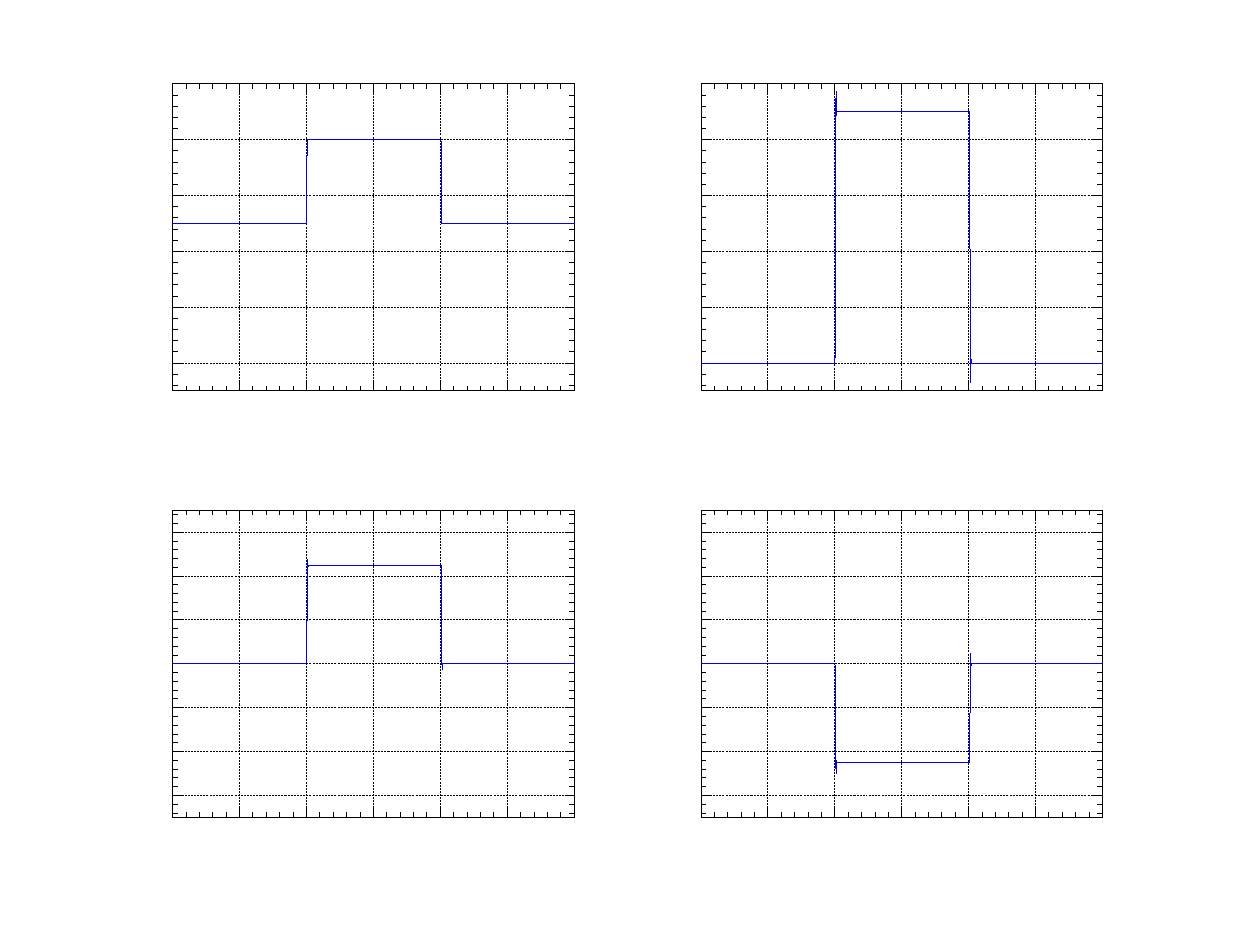
\includegraphics{DiffOutAmpTrans}}%
    \gplfronttext
  \end{picture}%
\endgroup
}
	\caption{Differential Output Amplifier transient response to a $0.2\unit{ms}$ pulse from a DAC output obtained using LTspice\textsuperscript{\textregistered}\label{fig:DiffAmpTransSim}}
	\end{singlespace}
\end{figure}
